\documentclass[12pt]{report}
\usepackage{amsmath,amssymb,amsfonts}
\usepackage{courier}
\usepackage{graphicx}
\usepackage{hyperref}
\usepackage{listings}
\usepackage{color}
\usepackage{tikz}
\usepackage{circuitikz}
\usetikzlibrary{shapes,arrows}
\usepackage[margin=2cm]{geometry}

\title{ECSE 426 - Microprocessor Systems\\Lab Report 2: Timers, Interrupts, Multithreaded, Interrupt-Driven Readings and Peripheral Control}
\author{Harley Wiltzer (260690006)\\Matthew Lesko (260692352)}
\date{March 19, 2018}

\definecolor{dblue}{rgb}{0.4,0.4,0.8}

\hypersetup {
	colorlinks=true,
	linkcolor=dblue
}

\tikzstyle{decision} = [diamond, draw, fill=blue!20, text badly centered, text width=2cm, node
distance=3cm]
\tikzstyle{block} = [rectangle, draw, fill=blue!20, text centered, rounded corners, minimum
height=4em, text width=3cm, node distance=5cm]
\tikzstyle{goal} = [rectangle, draw, fill=yellow!20, text centered, rounded corners, minimum
height=4em, text width=3cm, node distance=5cm]
\tikzstyle{line} = [draw, -latex']
\tikzstyle{cloud} = [draw, ellipse, fill=red!20, node distance=7cm, text centered, text width=2cm]
\tikzstyle{label} = [draw, rectangle, text centered, text width = 3cm]

\renewcommand*\thesection{\arabic{section}}

\begin{document}
\maketitle
\pagenumbering{roman}
\tableofcontents
%\let\clearpage\relax
\listoffigures
\let\clearpage\relax
\listoftables
\newpage
\pagenumbering{arabic}
\section{Abstract}
The purpose of experiment 3 is for the programmers to gain experience in utilizing timers and interrupts to accomplish a task which involves converting an analog pulse to digital and displaying its voltage on an LED display, effectively a voltmeter. The purpose of experiment 4 is for the programmers to gain exposure in designing a multithreaded application on a real time operating system (RTOS) running on an embedded system. The task of experiment 4 involves copying over experiment 3's program and subdiving several of its features each to its own concurrently running thread, with the goal of optimizing power usage. This report will explain in detail how the programmers implemented the problems stated below, as well as the challenges they faced, the testing they had done, and the conclusions they have made. By the end of the report, the reader shall understand how the timers available on the STM32F4 board can be used to activate peripherals and generate a pulse, and understand the implementation of multithreaded programs on embedded systems.
\section{Problem Statement}
The problem is for the developers to first implement a solution for generating a PWM pulse, whose voltage is set by an input on a keypad, that is then fed to a rectifier. Afterwards, the device shall feed the rectifier's output to an ADC to be converted to a digital signal, and have the signal's mean voltage be automatically displayed on an LED display. Furthermore, the program has to be implemented with the use of concurrently-running threads running on an RTOS. The problem can be divided into the following tasks:
\begin{itemize}
	\item Setting up a timer to act as a PWM pulse generator;
	\item Setting up a timer to activate the ADC to take an analog sample and convert it to digital;
	\item Designing a rectifier circuit component that takes the PWM pulse as input and feeds the output to the ADC;
	\item Testing and optimization of an FIR filter that reduces noise from the output signal of the ADC;
	\item Setting up the alphanumeric keypad so that the user may input their desired voltage to be displayed on an LED display;
	\item Mainting the 7-segment display;
	\item Coding a controller function that automates the changes to be made on the PWM's duty cycle so that the previous or default voltage updates to the target voltage on the LED display;
	\item Coding a finite state machine function that enables the user to Enter and Delete digits for the target voltage, Reset the target voltage, and put the device to Sleep by using the keypad;
	\item Implementating the program's features using CMSIS-RTOS and multithreading;
	\item Reducing the power consumption of the device when it is in sleep mode using CMSIS-RTOS.
\end{itemize}
\section{Theory and Hypothesis}
\subsection{Theory}
\subsection{Hypothesis}
\section{Implementation}
\subsection{Filtering}
The devices uses a modified FIR filter from experiment 2 [source] in order to reduce the noise of the ADC's signal. The two modifications are the following: 
\begin{itemize}
	\item Increasing from 5 coefficients to 10 being used in the moving average;
	\item Setting the first five coefficients to 0.05 and the last five coefficients to 0.15.
\end{itemize}
In this way, the 5 earliest samples hav have a significance of 0.05 and the 5 later samples have a significance of 0.15 when calculating the average of the 10 samples. The programmers drew this conclusion by trial and error and the empirical evidence proved that the above modifications to the FIR filter significantly reduced the signal's noise. The programmers have tested mutliple configurations, in which this report shall demonstrate three of them. One can draw comparisons from the following graphs generated by a run-time variables monitoring and visualization tool, STM Studio [source]:\\
\begin{figure}[h]
	\label{Linear Graph of the Filtered and Unfiltered Values Plotted Against Time}
	\begin{center}
		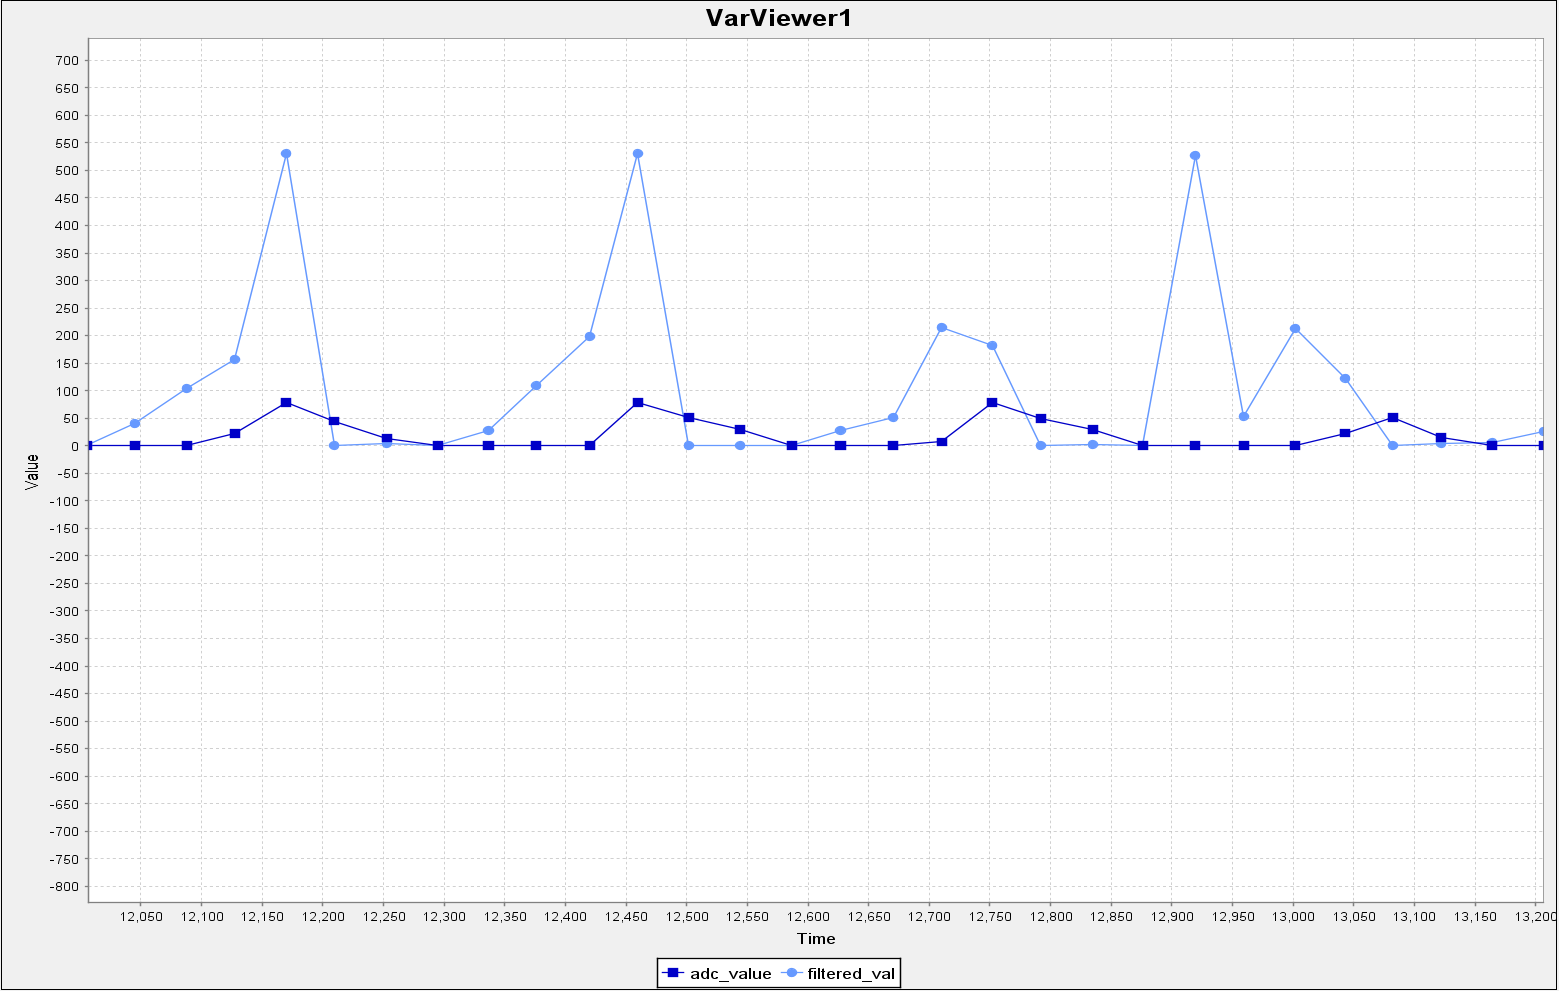
\includegraphics[scale=0.5]{./figures/adc_5coeffs.PNG}
		\caption{Filtered and Unfiltered Values VS Time (ms), Using Unmodified FIR Filter}
	\end{center}
\end{figure}
\\The configuration of this filter's coefficients is [0.2, 0.2, 0.2, 0.2, 0.2]. In regular blue are the unfiltered values, and in light blue are the filtered values. This graph demonstrates the values read at runtime of the unfilted and filtered values that passed through the unmodified FIR filter. One can observe that there is a considerable amount of noise left from filtering.
\begin{figure}[h]
	\label{Linear Graph of the Filtered and Unfiltered Values Plotted Against Time}
	\begin{center}
		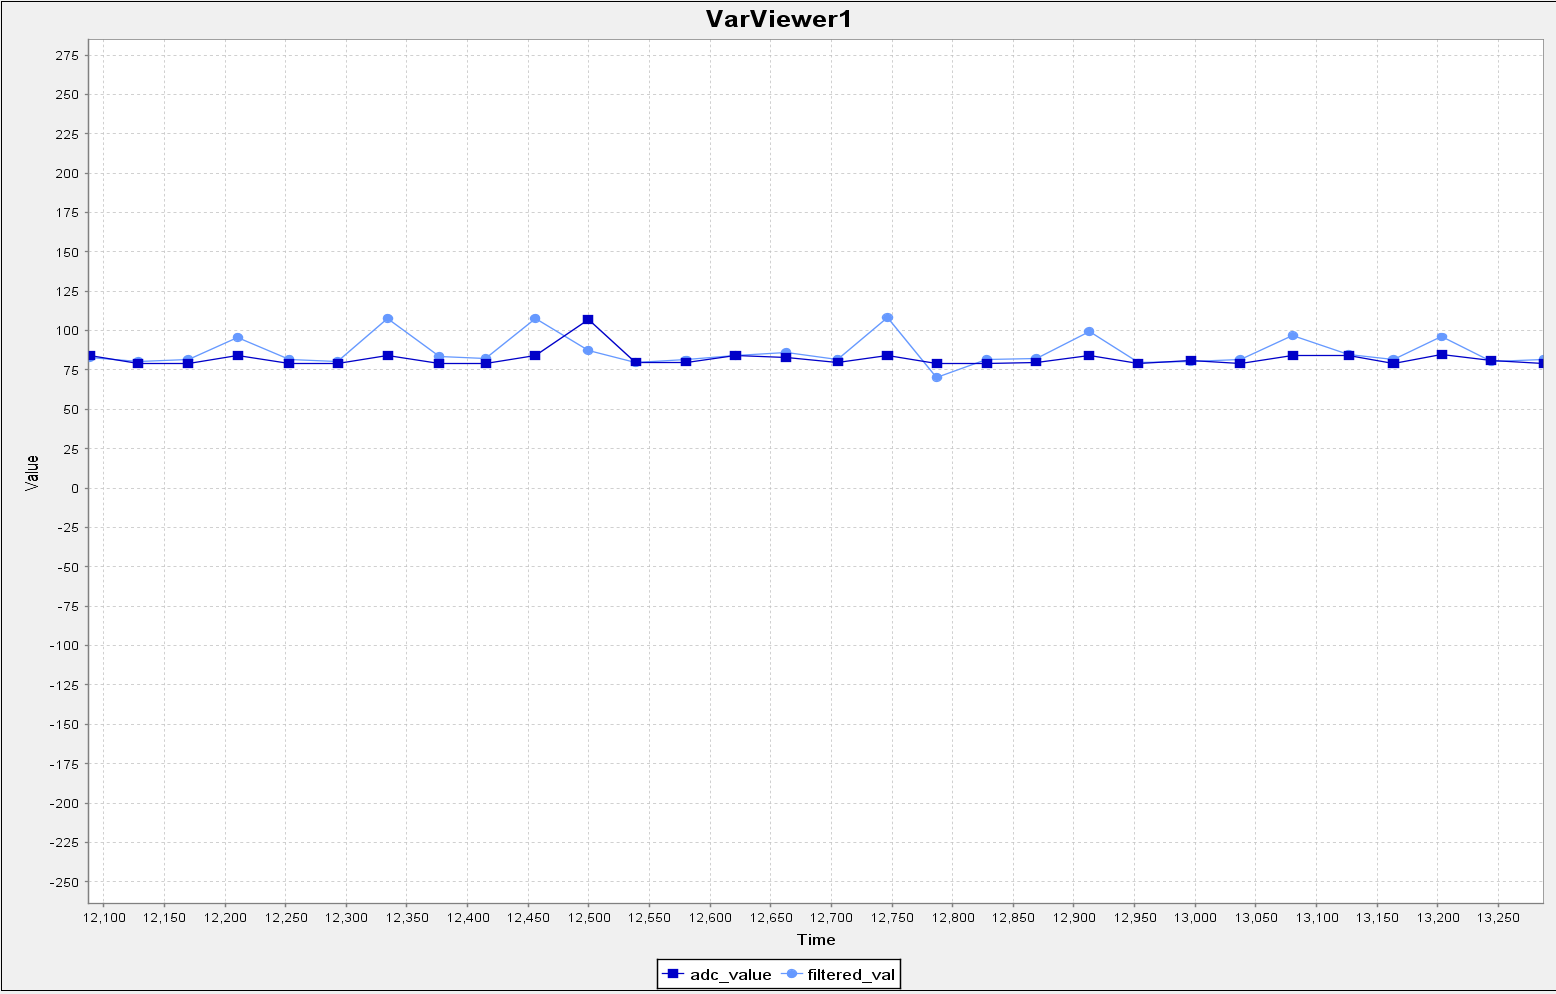
\includegraphics[scale=0.5]{./figures/adc_10coeffs_early_high_values.PNG}
		\caption{Filtered and Unfiltered Values VS Time (ms), Using High Coeffcients for Early Values}
	\end{center}
\end{figure}
\\The configuration of this filter's coefficients is [0.05, 0.05, 0.05, 0.05, 0.05, 0.15, 0.15, 0.15, 0.15, 0.15]. This filter considers the five earliest values to each have a significance of 0.15 and the five later values to each have a significance of 0.05. One can observe by the graph that this filter is a considerable improvement to the unmodified version. Although, the programmers believe that it could be optimized further.
\begin{figure}[h]
	\label{Linear Graph of the Filtered and Unfiltered Values Plotted Against Time}
	\begin{center}
		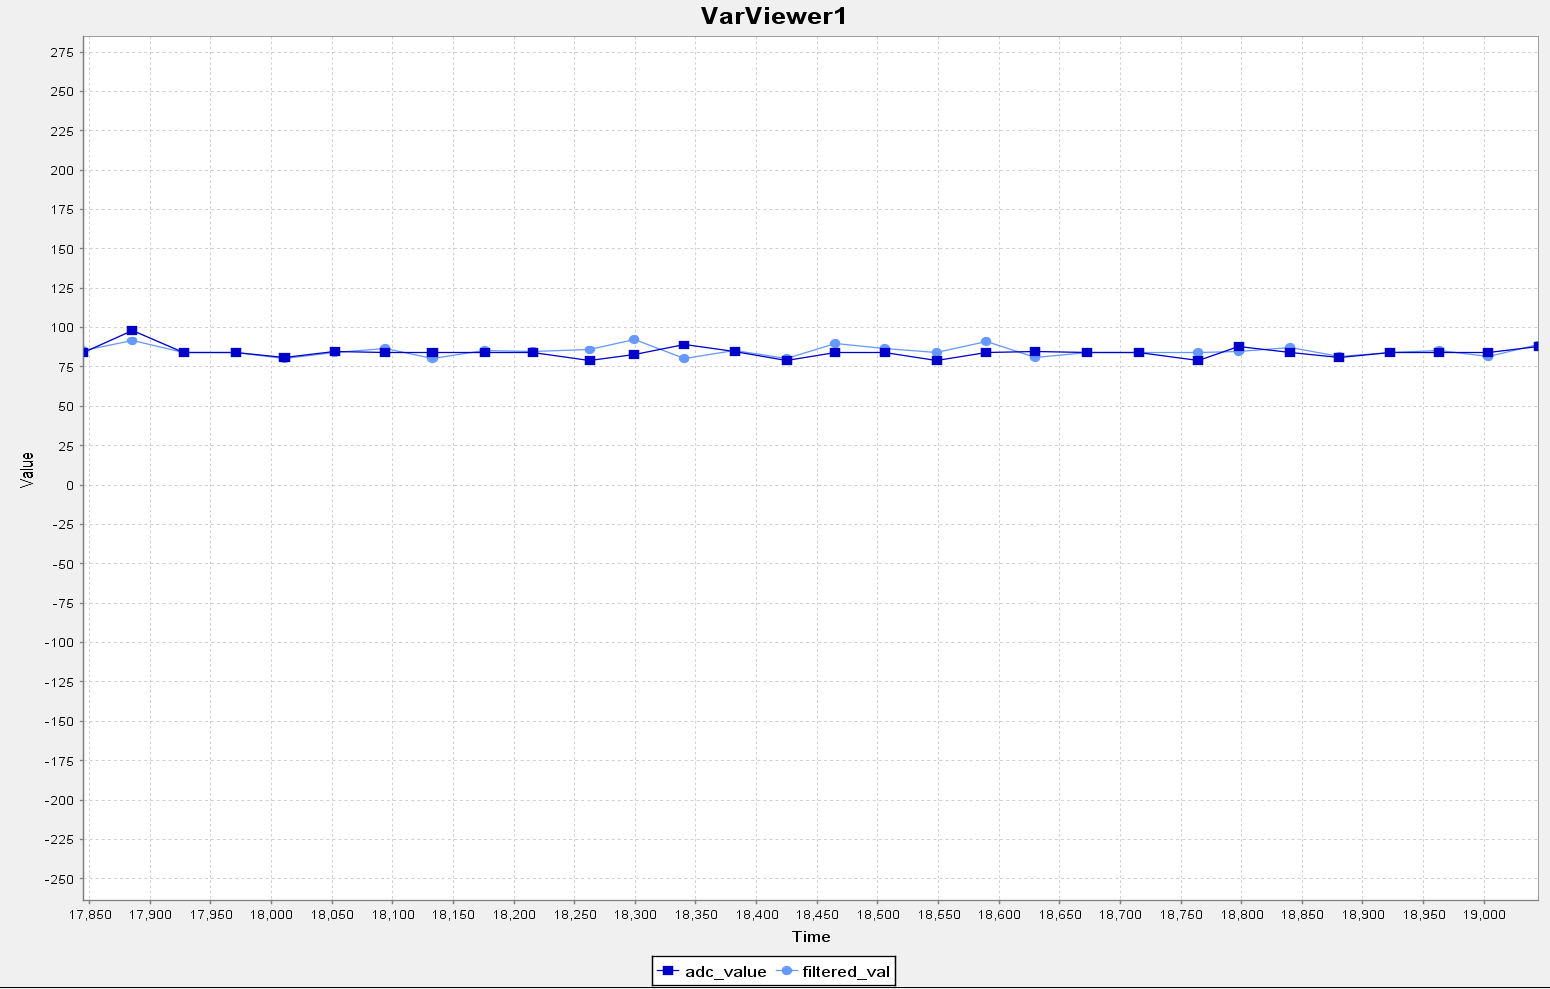
\includegraphics[scale=0.5]{./figures/adc_10coeffs_late_high_values.PNG}
		\caption{Filtered and Unfiltered Values VS Time (ms), Using High Coeffcients for Late Values}
	\end{center}
\end{figure}
\\The configuration of this filter's coefficients is [0.15, 0.15, 0.15, 0.15, 0.15, 0.05, 0.05, 0.05, 0.05, 0.05]. This filter considers the five later values to each have a significance of 0.15 and the five early values to each have a significance of 0.05. One can observe by the graph that this filter is an improvement to the previous version. The programmers believe that this version of the filter should perform well enough given the scope of the problem.

\section{Testing and Observations}
\section{Conclusion}
\newpage
\begin{appendix}\label{appendices}
	\chapter{GPIO Configuration Parameters}\label{appendixgpio}
	This appendix lists the configuration parameters set for each of the different GPIO pins (or
	classes of GPIO pins).\\\\
	\textbf{User Input Button}\\
	\begin{tabular}{|c|c|}
		\hline
		Parameter & Value\\\hline
		Mode & \texttt{GPIO\_MODE\_IT\_RISING}\\\hline
		Pull & \texttt{GPIO\_NOPULL}\\\hline
	\end{tabular}
	\newline
	\\\\
	\textbf{Display Mode LEDs (4 of these)}\\
	\begin{tabular}{|c|c|}
		\hline
		Parameter & Value\\\hline
		Mode & \texttt{GPIO\_MODE\_OUTPUT\_PP}\\\hline
		Pull & \texttt{GPIO\_NOPULL}\\\hline
		Speed & \texttt{GPIO\_SPEED\_FREQ\_LOW}\\\hline
	\end{tabular}
	\newline
	\\\\
	\textbf{Display Segment Pins (8 of these)}\\
	\begin{tabular}{|c|c|}
		\hline
		Parameter & Value\\\hline
		Mode & \texttt{GPIO\_MODE\_OUTPUT\_PP}\\\hline
		Pull & \texttt{GPIO\_NOPULL}\\\hline
		Speed & \texttt{GPIO\_SPEED\_FREQ\_LOW}\\\hline
	\end{tabular}
	\newline
	\\\\
	\textbf{Display Selector Pins (3 of these)}\\
	\begin{tabular}{|c|c|}
		\hline
		Parameter & Value\\\hline
		Mode & \texttt{GPIO\_MODE\_OUTPUT\_PP}\\\hline
		Pull & \texttt{GPIO\_NOPULL}\\\hline
		Speed & \texttt{GPIO\_SPEED\_FREQ\_LOW}\\\hline
	\end{tabular}
	\newline
	\newpage
	\chapter{ADC Configuration Settings}\label{appendixadc}
	\textbf{ADC Instance Parameters}\\
	\begin{tabular}{|c|c|}
		\hline
		Parameter & Value\\\hline
		Clock Prescaler & \texttt{ADC\_CLOCK\_SYNC\_PCLK\_DIV2}\\\hline
		Resolution & \texttt{ADC\_RESOLUTION\_8B}\\\hline
		Scan Conversion Mode & Disabled\\\hline
		Continuous Conversion Mode & Disabled\\\hline
		Discontinuous Conversion Mode & Disabled\\\hline
		External Trigger Conversion Edge & \texttt{ADC\_EXTERNALTRIGCONVEDGE\_RISING}\\\hline
		External Trigger Conversion & \texttt{ADC\_SOFTWARE\_START}\\\hline
		Data Alignment & \texttt{ADC\_DATAALIGN\_RIGHT}\\\hline
		Number of Conversions & 1\\\hline
		DMA Continuous Requests & Disabled\\\hline
		EOC Selection & \texttt{ADC\_EOC\_SINGLE\_CONV}\\\hline
	\end{tabular}
	\newline
	\\\\
	\textbf{ADC Channel Parameters (Channel 1)}\\
	\begin{tabular}{|c|c|}
		\hline
		Parameter & Value\\\hline
		Rank & 1\\\hline
		Sampling Time & \texttt{ADC\_SAMPLETIME\_3CYCLES}\\\hline
	\end{tabular}
	\newpage
	\chapter{HAL Cube MX Autogenerated Code}\label{mammoth}
	\begin{lstlisting}[basicstyle=\scriptsize\ttfamily]
	\end{lstlisting}
	
	\newpage
	\chapter{Theory References}
\end{appendix}
\end{document}
